%% Direttive TeXworks:
% !TeX root = ../report.tex
% !TEX encoding = UTF-8 Unicode
% !TeX spellcheck = it-IT

% arara: pdflatex: { synctex: yes, shell: yes, interaction: nonstopmode }
% arara: bibtex
% arara: pdflatex: { synctex: yes, shell: yes, interaction: nonstopmode }
% arara: pdflatex: { synctex: yes, shell: yes, interaction: nonstopmode }

Essendo lo Sprint iniziale, è stata realizzata un'attenta analisi di tutti i requisiti forniti dal committente
con uno sguardo generale su tutto il sistema, in modo da poter chiarire con quest'ultimo eventuali incomprensioni.

L'obiettivo di questo primo Sprint è individuare struttura e interazioni di massima del sistema; in particolare:
\begin{itemize}
  \item
    con l'analisi dei requisiti si vuole far emergere i componenti del sistema del committente;
  \item
    con l'analisi del problema si vuole identificare eventuali ulteriori componenti di interesse per la futura progettazione;
  \item
    con la fase di progettazione si vuole decidere a livello più basso le scelte tecnologiche e come procedere per la stesura del codice.
\end{itemize}

Una volta formalizzata un prima analisi dei requisiti generale, reperibile in questo documento alla \Cref{sec:req_analysis},
il passo successivo è individuare i requisiti prioritari da realizzare in questo primo Sprint, in modo da poterli analizzare nel dettaglio.

\subsection{Analisi dei requisiti}\labelssec{sp1:req_analysis}

Dopo aver delineato tutti i requisiti base, si è scelto di approfondire quelli maggiormente fondanti e di valore per il prodotto:

\begin{description}[itemsep=1em]
  \item[\requirementref{R-startExplore}]
    tramite una console grafica l'utente dovrà poter inviare un comando di inizio esplorazione, il comando dovrà essere ricevuto dal robot, il quale dovrà dare inizio alla fase di esplorazione se il requisito successivo è verificato.
  \item[\requirementref{R-explore}]
    l'esplorazione per questo sprint iniziale sarà dummy, in modo da permettere all'utente di vedere il robot muoversi.
  \item[\requirementref{R-tempOk}]
    l'esplorazione dovrà partire soltanto se la temperatura è inferiore ad una certa soglia.
    Da requisiti iniziali non è chiaro se il robot debba essere reattivo a cambi della temperatura durante la fase di esplorazione;
    per il momento si assume di no.
  \item[\requirementref{R-stopExplore}]
    in seguito ad un comando dell'utente l'esplorazione dovrà essere interrotta ed il robot rimarrà in attesa di sapere dall'utente se deve tornare a casa oppure proseguire l'esplorazione appena interrotta.
  \item[\requirementref{R-continueExplore}]
    se l'utente ha inviato il comando per riprendere l'esplorazione il robot deve riprenderla.
  \item[\requirementref{R-backHome}]
    se invece l'utente ha deciso che il robot debba tornare alla sua base, il robot deve farlo.
    Si specifica però che in questo primo sprint non essendo stato ancora introdotto il concetto di mappa, dunque il ritorno a casa sarà soltanto simulato.
\end{description}

Il prodotto dell'analisi dei requisiti deve essere una prima versione dell'architettura logica, che modelli e rappresenti formalmente i requisiti del sistema.

\subsection{Metamodello e QA}\labelssec{qa}

Per rappresentare in maniera formale l'architettura logica, si è scelto di utilizzare il meta-linguaggio QA, nella sua versione \textbf{1.5.13.2}.
Questo linguaggio è stato messo a disposizione dalla software house e permette di superare le limitazioni intrinseche della modellazione UML
(principalmente object-oriented e con notevoli limitazioni nel distribuito).

Il linguaggio QA è adatto per costruire modelli eseguibili di sistemi software e permette di generare rappresentazioni grafiche del sistema,
permettendo di facilitare la comprensione di \textbf{struttura}, \textbf{interazione} e \textbf{comportamento} dello stesso.

\begin{figure}[H]
  \centering
  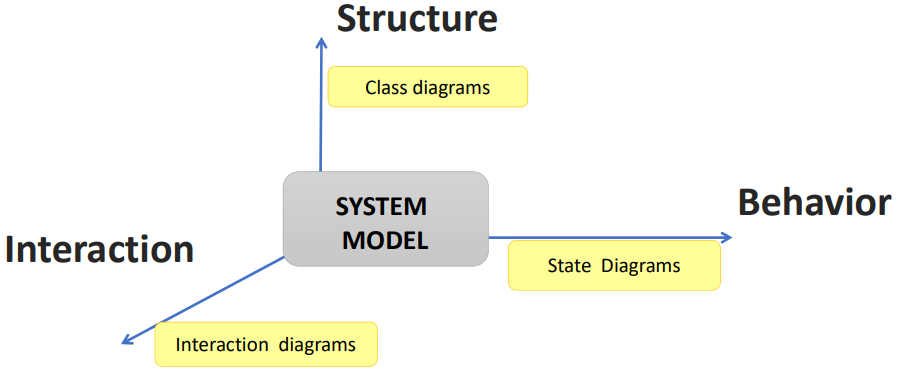
\includegraphics[width=1\textwidth]{res/logicalArchitecture.png}%
  \label{fig:logicalArchitecture}
\end{figure}

\subsection{Architettura logica in output all'analisi dei requisiti}\labelssec{sp1:arch_logica_req}

Partendo con un approccio top-down, sono stati prima di tutto riconosciuti i 3 componenti principali:

\begin{figure}[H]
  \centering
  \includegv[width=1\textwidth]{res/sprint1/requirements/console}
  \caption{Console}%
  \label{fig:sp1:req:console}
\end{figure}

\begin{figure}[H]
  \centering
  \includegv[width=1\textwidth]{res/sprint1/requirements/robotdiscovery}
  \caption{Robot Discovery}%
  \label{fig:sp1:req:robotdiscovery}
\end{figure}

\begin{figure}[H]
  \centering
  \includegv[width=1\textwidth]{res/sprint1/requirements/robotretrieval}
  \caption{Robot Retrieval}%
  \label{fig:sp1:req:robotretrieval}
\end{figure}

Analizzando i tipi di interazioni, si è deciso che queste ultime funzionano come seguono:

\begin{itemize}
  \item
    Il robot invia informazioni sullo stato alla console tramite l'invio di messaggi di tipo \textbf{fire-and-forget}
    (\texttt{dispatch} nel meta-linguaggio QA).

    Essendo il tipo di interazione \textit{uno-ad-uno}, si è ritenuto appropriato utilizzare come metodo di interazione lo scambio di messaggi.

  \item
    La console invia istruzioni ai robot anch'essa tramite l'invio di messaggi;
    le ragioni sono analoghe al caso precedente,
    e a maggior ragione è evidente come vi sia uno e soltanto un destinatario.

\end{itemize}

\clearpage

Di seguito è riportata la prima versione dell'architettura logica in output all'analisi dei requisiti formalizzata tramite metamodello QA\@.

\lstinputlisting[language=qa]{res/sprint1/requirements/robot.qa}

\subsection{Analisi del problema}\labelssec{sp1:prob_analysis}

Durante la fase di analisi del problema si è deciso di dividere il \textbf{robot discovery} in due componenti principali:

\begin{itemize}
  \item uno che conterrà la business logic (\textbf{robot-mind}).
  \item uno che lavorerà come adattatore per i robot in ambiente virtuale o fisico (\textbf{robot-adapter}).
\end{itemize}

Inoltre è stato aggiunto un componente che si occupa di valutare se le condizioni per il funzionamento del robot siano favorevoli o meno e di informare la \textbf{robot-mind}.

\subsubsection{World observer}\labelsssec{sp1:world_observer}

Dato che le informazioni ambientali vengono generate esternamente sia rispetto al robot che rispetto alla console,
è stato ritenuto approriato istruire un nuovo componente nel sistema che si occupi di osservare le variazioni delle condizioni ambientali
e che vada a valutarle per decidere se queste sono favorevoli o meno al corretto funzionamento del robot (\requirementref{R-tempOk});
una volta valutate tali condizioni, il componente emette un evento tramite il quale informa il resto del sistema.

\subsubsection{Robot Adapter e Robot Mind}\labelsssec{sp1:mind_adapter}

Si è ritenuto opportuno separare la logica di funzionamento del robot dal componente che si occupa di eseguire le istruzioni per vari motivi,
tra cui ottenere una maggiore separazione tra un componente chiave contenente la \textbf{business logic}, core del sistema, (\textbf{robot-mind}) ed un mero esecutore di comandi (\textbf{robot-adapter}).
Tra l'altro questo permette di mantenere un certo livello di \textbf{technology independency} e \textbf{riusabilità} nel sistema.

Il robot-adapter altro non è che un \textbf{driver} che esegue i comandi ricevuti dalla \textbf{mind} nel mondo fisico o in quello virtuale (o in entrambi) e non deve sapere nulla della logica di funzionamento del sistema.

\subsection{Architettura logica in output all'analisi del problema}\labelssec{sp1:arch_logica_prob}

Procedendo con un approccio top-down, a seguito dello zoom-in sono stati identificati i seguenti componenti:

\begin{figure}[H]
  \centering
  \includegv[width=0.6\textwidth]{res/sprint1/problem/world_observer}
  \caption{World Observer}%
  \label{fig:sp1:prob:worldobserver}
\end{figure}

\begin{figure}[H]
  \centering
  \includegv[width=1\textwidth]{res/sprint1/problem/robot_adapter}
  \caption{Robot Adapter}%
  \label{fig:sp1:prob:robotadapter}
\end{figure}

\begin{figure}[H]
  \centering
  \includegv[width=1\textwidth]{res/sprint1/problem/robot_retriever_mind}
  \caption{Robot Retrieval Mind}%
  \label{fig:sp1:prob:robotretrieval}
\end{figure}

\begin{figure}[H]
  \centering
  \includegv[width=1.2\textwidth]{res/sprint1/problem/robot_discovery_mind}
  \caption{Robot Discovery Mind}%
  \label{fig:sp1:prob:robotdiscovery}
\end{figure}

\begin{figure}[H]
  \centering
  \includegv[width=1\textwidth]{res/sprint1/problem/console}
  \caption{Console}%
  \label{fig:sp1:prob:console}
\end{figure}

Procedendo con l'analisi delle interazioni, sono state effettuate le seguenti modifiche:
\begin{itemize}
    \item
      I comandi ricevuti dal \textbf{robot adapter} possono essere \textbf{messaggi};
      questo è dovuto al fatto che il robot potrebbe ricevere comandi urgenti ed è fondamentale che vengano effettivamente elaborati;
    \item
      Il \textbf{world observer} osserva le condizioni ambientali notificate tramite \textbf{eventi} e,
      dopo aver operato le sue valutazioni, emette anch'esso degli eventi per informare il resto del sistema che le condizioni sono favorevoli o avverse.
      Infatti non è necessario notificare di ciò uno specifico componente del sistema, né è necessaria alcuna forma di garanzia sul fatto che prima o poi queste informazioni vengano elaborate.
\end{itemize}

\subsection{Software già disponibile}\labelssec{sp1:avail_sw}

Nella fase di analisi del problema, l'approccio top-down deve andare parzialmente incontro all'approccio bottom-up:
la software house, infatti, fornisce alcuni componenti tecnologici già realizzati ed è consigliabile appoggiarsi ad essi per realizzare alcuni componenti del sistema:

\begin{itemize}
    \item il \textbf{robot adapter} deve quindi occuparsi di adattare il robot che ci viene fornito (fisico o virtuale), alla struttura modellata nel sistema;
    \item la \textbf{console} si occupa invece di adattare l'interfaccia grafica messa a disposizione dal framework QA (WebGUI) alla console specificata dai requisiti.
\end{itemize}

\subsection[Rappresentazione formale]{Rappresentazione formale in output alla fase di analisi del problema}\labelssec{sp1:qa}

Di seguito è riportata la versione finale per lo Sprint 1 dell'architettura logica in output all'analisi del problema formalizzata tramite metamodello QA\@.

\lstinputlisting[language=qa]{res/sprint1/problem/robot.qa}

\subsection{Progettazione e Test planning}\labelssec{sp1:project}

In questa fase sono state progettate le soluzioni alle problematiche individuate nelle fasi precedenti.

Per quanto riguarda la progettazione della struttura del sistema, si è scelto di utilizzare la struttura suggerita dal framework QA, in quanto ritenuta adeguata a quanto richiesto.
In particolare, il fatto che si basi su pattern architetturale MVC permette di intervenire più facilmente sui singoli moduli, potendone cambiare il comportamento senza dover effettuare modifiche troppo onerose.

La scelta di questo modulo comporta inoltre l'utilizzo futuro della tecnologia \textbf{MQTT} come protocollo \textit{publish/subscribe} e di \textbf{Akka} per lo \textit{scambio di messaggi} tra gli attori,
vincolo che non comporta eccessivi problemi di progettazione per il fatto che i QA possiedono nativamente un supporto per la comunicazione \textit{publish/subscribe}.

Al fine di velocizzare i tempi di realizzazione del sistema, evitando di dover affrontare problematiche relative al robot fisico,
è stato utilizzato, per questo primo sprint, un robot demo mock e il robot virtuale a dispoizione, realizzando comunque il sistema in modo che l'utilizzo del robot fisico potesse essere effettuato con sforzo esiguo.

Per quanto rigurarda il test planning, si intende realizzare test automatizzati solo per alcuni dei requisiti da soddisfare, cioé quelli per i quali l'esecuzione di una demo non è sufficiente a comprenderne il corretto funzionamento.

Per svolgere i test si intende utilizzare \texttt{QActorUtils}, modulo di supporto fornito dalla software house che permette di ispezionare la base di conoscenza interna, ottenere i riferimenti e mandare messaggi ai QActors di un determinato contesto;
in questo modo, è possibile realizzare test JUnit verificabili tramite CI (come Travis CI) o IDE (come Eclipse).

È evidente come i test automatici siano parziali e non esaustivi, ma possono essere di aiuto per testare l'interazione ed il comportamento complessivo del sistema.
Per la natura dei requisiti è stato possibile automatizzare i seguenti test per i requisiti:

\begin{description}
  \item[TestRBlinkLed]
    si vuole accertare che se il robot è in fase di esplorazione il LED lmapeggi, mentre se è fermo allora il LED sia spento.
  \item[TestROkTemperature]
    viene testato che se la temperatura è superiore alla soglia, il worldobserver se ne accorge e sa che lo stato dell'ambiente non è adeguato.
\end{description}

Per quanto riguarda gli altri requisiti, gli unici test che sono stati condotti sono di tipo qualitativo, osservando l'esecuzione di un sistema mock valutando i casi di utilizzo.

In questo caso, il monitoring è stato effettuato sfruttuando l'interfaccia Web e i log sulla console.
